% Created 2023-03-06 Mon 15:36
% Intended LaTeX compiler: pdflatex
\documentclass[presentation, aspectratio=1610]{beamer}
\usepackage[utf8]{inputenc}
\usepackage[T1]{fontenc}
\usepackage{graphicx}
\usepackage{longtable}
\usepackage{wrapfig}
\usepackage{rotating}
\usepackage[normalem]{ulem}
\usepackage{amsmath}
\usepackage{amssymb}
\usepackage{capt-of}
\usepackage{hyperref}
\usetheme[progressbar=foot]{metropolis}
\usepackage{caption}
\captionsetup[figure]{labelformat=empty}
\AtBeginSubsection{\begin{frame}\tableofcontents[currentsection,currentsubsection]\end{frame}}
\usetheme{metropolis}
\usecolortheme{}
\usefonttheme{}
\useinnertheme{}
\useoutertheme{}
\author{Andrew Jensen}
\date{March 9, 2023}
\title{Joint Track Machine Learning}
\hypersetup{
 pdfauthor={Andrew Jensen},
 pdftitle={Joint Track Machine Learning},
 pdfkeywords={},
 pdfsubject={},
 pdfcreator={Emacs 28.1 (Org mode 9.6)}, 
 pdflang={English}}
\usepackage{biblatex}
\addbibresource{/home/andrew/repo/lit-review/src/myBib.bib}
\addbibresource{~/org/biblio.bib}
\begin{document}

\maketitle
\begin{frame}{Outline}
\tableofcontents
\end{frame}


\section{Introduction}
\label{sec:org90aff05}
\begin{frame}[label={sec:org8ac3493}]{Acknowledgments}
I would like to thank the McJunkin Family Charitable Foundation for their generous grant that supports this work.
\end{frame}
\section{Motivation}
\label{sec:org174cea0}
\begin{frame}[label={sec:orgf1a3c16}]{The Problem}
\begin{columns}
\begin{column}{0.5\columnwidth}
\begin{itemize}
\item By 2030, roughly 3.5 million Total Knee Arthroplasty (TKA) will be performed in the US \autocite{kurtzProjectionsPrimaryRevision2007}.
\item 20\% of patients receiving TKA are dissatisfied.
\begin{itemize}
\item Instability, pain, unnatural \autocites{bakerRolePainFunction2007}[][]{bournePatientSatisfactionTotal2010}[][]{scottPredictingDissatisfactionFollowing2010}.
\end{itemize}
\item No reliable method of clinically assessing and quantifying joint dynamics.
\begin{itemize}
\item Too much human supervision, too time consuming
\end{itemize}
\end{itemize}
\end{column}
\begin{column}{0.5\columnwidth}
\begin{center}
\includegraphics[width=\textwidth]{/home/andrew/repo/lit-review/figures/raster/Physical_Examination_of_the_knee.jpg}
\end{center}
\end{column}
\end{columns}
\end{frame}
\begin{frame}[label={sec:orge11abe5}]{Our Proposition}
\begin{columns}
\begin{column}{0.5\columnwidth}
Orthopaedic surgeons and clinicians would readily adopt a \alert{\alert{practical}} and \alert{\alert{inexpensive}} technology that allows them to \alert{\alert{measure}} a patient's knee kinematics during \alert{\alert{activities of daily living}}.
\end{column}
\begin{column}{0.55\columnwidth}
\begin{center}
\includegraphics[width=2in]{/home/andrew/repo/lit-review/figures/raster/dynamic-knee-prescription.png}
\end{center}
\end{column}
\end{columns}
\end{frame}
\begin{frame}[label={sec:org81ac375}]{Constraints}
\begin{columns}
\begin{column}{0.45\columnwidth}
\begin{itemize}
\item It must fit within a \alert{\alert{standard clinical workflow}}
\item The technology must utilize equipment \alert{\alert{commonly found in hospitals}}
\item There must not be significant \alert{\alert{human supervision}} nor interaction to generate an examination report.
\end{itemize}
\end{column}
\begin{column}{0.55\columnwidth}
\begin{center}
\includegraphics[width=\textwidth]{/home/andrew/repo/lit-review/figures/raster/c-arm-fluoro-machine.jpg}
\end{center}
\end{column}
\end{columns}
\end{frame}
\section{Background}
\label{sec:orge068d6d}
\begin{frame}[label={sec:orge12b789}]{Projective Geometry}
\begin{columns}
\begin{column}{0.5\columnwidth}
\begin{equation*}
  \begin{pmatrix}
    x_{s} \\ y_{s} \\ z_{s} \\ 1
  \end{pmatrix}_{i} = T^{cam}_{scene} \mathbf{\tilde{p}^{obj}_{i}}
\end{equation*}

\begin{equation*}
  \begin{pmatrix}
    \tilde{x}_{img} \\ \tilde{y}_{img} \\ \tilde{z}
  \end{pmatrix} =
  \begin{pmatrix}
    f& 0 & 0 \\ 0 & f & 0 \\ 0 & 0 & 1
  \end{pmatrix} \vec{x}_{s}
\end{equation*}

Where
\begin{equation*}
  \begin{aligned}
    x_{img} &= \frac{\tilde{x_{img}}}{\tilde{z}} = \frac{f}{z_{s}}x_{s} \\
    y_{img} &= \frac{\tilde{y_{img}}}{\tilde{z}} = \frac{f}{z_{s}}y_{s}
  \end{aligned}
\end{equation*}

{\tiny Note: We are still in the camera's reference frame}
\end{column}

\begin{column}{0.6\columnwidth}
\begin{center}
\includegraphics[width=.9\linewidth]{/home/andrew/repo/lit-review/figures/raster/perspective-projection.png}
\end{center}
\end{column}
\end{columns}
\end{frame}
\begin{frame}[label={sec:org5cc1d08}]{Projective Geometry}
\begin{center}
\includegraphics[width=.9\linewidth]{/home/andrew/repo/lit-review/figures/raster/perspective-projection.png}
\end{center}
\end{frame}
\begin{frame}[label={sec:org392278b}]{Pixel Coordinates}
Convert camera coordinates into image coordinates.
\begin{equation*}
  \begin{aligned}
    p_{x} = k_{x}x_{img} + c_{x} \\
    p_{y} = k_{y}y_{img} + c_{y}
  \end{aligned}
\end{equation*}
Where
\begin{equation*}
  \begin{aligned}
    k &\equiv \text{ Pixel Spacing }\\
    c &\equiv \text{ Image Focal Point }
  \end{aligned}
\end{equation*}
\end{frame}

\begin{frame}[label={sec:org1fb4f11}]{Model-Image Registration}
\begin{columns}
\begin{column}{0.5\columnwidth}
If we know the projective parameters of the fluoroscopy machine, can we tinker with \(T^{cam}_{implant}\) so that our virtual projection matches the fluoroscopic image?
\end{column}
\begin{column}{0.6\columnwidth}
\begin{figure}[htbp]
\centering
\includegraphics[width=2.5in]{/home/andrew/repo/lit-review/figures/raster/mahfouz-perspective-projection.png}
\caption{From \autocite{mahfouzRobustMethodRegistration2003}}
\end{figure}
\end{column}
\end{columns}
\end{frame}
\section{Historical Methods}
\label{sec:org733ecda}
\begin{frame}[label={sec:org0db7101}]{Overview}
Many different approaches have attempted to solve the model-image registration problem.
\begin{itemize}
\item Pre-computed projections
\item Skin-mounted motion Capture
\item Biplane Imaging
\item Iterative Projections
\item Model-based Roentgen Stereophotogrammetry
\end{itemize}
\end{frame}
\begin{frame}[label={sec:org9ef2007}]{Pre-Computed Projections}
\begin{columns}
\begin{column}{0.5\columnwidth}
\begin{itemize}
\item Saving space and memory by pre-computing as much as possible.
\item Pre-computed distance maps \autocites{zuffiModelbasedMethodReconstruction1999}[][]{lavalleeRecoveringPositionOrientation1995}.
\item Pre-computed shape libraries \autocite{banksAccurateMeasurementThreedimensional1996}
\end{itemize}
\end{column}
\begin{column}{0.6\columnwidth}
\begin{figure}[htbp]
\centering
\includegraphics[width=1.75in]{/home/andrew/repo/lit-review/figures/raster/lavallee-distance-maps.png}
\caption{From \autocite{lavalleeRecoveringPositionOrientation1995}}
\end{figure}
\vspace{-0.25in}
\begin{figure}[htbp]
\centering
\includegraphics[width=1.75in]{/home/andrew/repo/lit-review/figures/raster/banks-nfd-library.png}
\caption{From \autocite{banksAccurateMeasurementThreedimensional1996}}
\end{figure}
\end{column}
\end{columns}
\end{frame}
\begin{frame}[label={sec:orgc52ff3d}]{Limitations of Pre-Computed Projections}
\begin{columns}
\begin{column}{0.5\columnwidth}
\begin{itemize}
\item Requires an accurate contour from the input image in order to perform calculations.
\end{itemize}
\end{column}
\begin{column}{0.6\columnwidth}
\begin{figure}[htbp]
\centering
\includegraphics[width=1.75in]{/home/andrew/repo/lit-review/figures/raster/lavallee-distance-maps.png}
\caption{From \autocite{lavalleeRecoveringPositionOrientation1995}}
\end{figure}
\vspace{-0.25in}
\begin{figure}[htbp]
\centering
\includegraphics[width=1.75in]{/home/andrew/repo/lit-review/figures/raster/banks-nfd-library.png}
\caption{From \autocite{banksAccurateMeasurementThreedimensional1996}}
\end{figure}
\end{column}
\end{columns}
\end{frame}

\begin{frame}[label={sec:org0b90d2e}]{Motion Capture (MoCap)}
\begin{columns}
\begin{column}{0.5\columnwidth}
\begin{itemize}
\item Can measure motion of MoCap beads very accurately.
\item Skin-mounted \autocites{gaoInvestigationSoftTissue2008}[][]{kuoInfluenceSoftTissue2011}[][]{linEffectsSoftTissue2016}.
\item Bone pins \autocite{lafortuneThreedimensionalKinematicsHuman1992} (any volunteers?).
\end{itemize}
\end{column}

\begin{column}{0.6\columnwidth}
\begin{figure}[htbp]
\centering
\includegraphics[width=2.5in]{/home/andrew/repo/lit-review/figures/raster/gao-skin-mocap.png}
\caption{From \autocite{gaoInvestigationSoftTissue2008}}
\end{figure}
\vspace{-0.25in}
\begin{figure}[htbp]
\centering
\includegraphics[width=2.5in]{/home/andrew/repo/lit-review/figures/raster/lafortune-bone-mocap.png}
\caption{From \autocite{lafortuneThreedimensionalKinematicsHuman1992}}
\end{figure}
\end{column}
\end{columns}
\end{frame}
\begin{frame}[label={sec:orgb06ec3d}]{Limitations of Motion Capture}
\begin{columns}
\begin{column}{0.5\columnwidth}
Skin Mounted
\begin{itemize}
\item Doesn't accurately describe underlying skeletal motion with clinical accuracy \autocites{gaoInvestigationSoftTissue2008}[][]{kuoInfluenceSoftTissue2011}[][]{linEffectsSoftTissue2016}.
\end{itemize}
Bone Pins
\begin{itemize}
\item Bone Pins
\item Need I say more?
\end{itemize}
\end{column}

\begin{column}{0.6\columnwidth}
\begin{figure}[htbp]
\centering
\includegraphics[width=2.5in]{/home/andrew/repo/lit-review/figures/raster/gao-skin-mocap.png}
\caption{From \autocite{gaoInvestigationSoftTissue2008}}
\end{figure}
\vspace{-0.25in}
\begin{figure}[htbp]
\centering
\includegraphics[width=2.5in]{/home/andrew/repo/lit-review/figures/raster/lafortune-bone-mocap.png}
\caption{From \autocite{lafortuneThreedimensionalKinematicsHuman1992}}
\end{figure}
\end{column}
\end{columns}
\end{frame}

\begin{frame}[label={sec:orgd2b8c11}]{Biplane Imaging}
\begin{columns}
\begin{column}{0.5\columnwidth}
\begin{itemize}
\item Utilizes multiple cameras to resolve 3D position and orientation\autocites{ivesterReconfigurableHighSpeedStereoRadiography2015}[][]{burtonAutomaticTrackingHealthy2021}.
\begin{itemize}
\item Highly accurate.
\item Gold Standard.
\end{itemize}
\end{itemize}
\end{column}
\begin{column}{0.6\columnwidth}
\begin{figure}[htbp]
\centering
\includegraphics[width=1.75in]{/home/andrew/repo/lit-review/figures/raster/ivester-stereo-fluoromachine.png}
\caption{Both from \autocite{ivesterReconfigurableHighSpeedStereoRadiography2015}}
\end{figure}
\vspace{-0.25in}
\begin{figure}[htbp]
\centering
\includegraphics[width=1.75in]{/home/andrew/repo/lit-review/figures/raster/ivester-stereo-projection.png}
\end{figure}
\end{column}
\end{columns}
\end{frame}
\begin{frame}[label={sec:org8ef4eb6}]{Limitations of Biplane Imaging}
\begin{columns}
\begin{column}{0.5\columnwidth}
\begin{itemize}
\item Not many hospitals have biplane fluoroscopy setups.
\item Clinically impractical
\end{itemize}
\end{column}
\begin{column}{0.6\columnwidth}
\begin{figure}[htbp]
\centering
\includegraphics[width=1.75in]{/home/andrew/repo/lit-review/figures/raster/ivester-stereo-fluoromachine.png}
\caption{Both from \autocite{ivesterReconfigurableHighSpeedStereoRadiography2015}}
\end{figure}
\vspace{-0.25in}
\begin{figure}[htbp]
\centering
\includegraphics[width=1.75in]{/home/andrew/repo/lit-review/figures/raster/ivester-stereo-projection.png}
\end{figure}
\end{column}
\end{columns}
\end{frame}

\begin{frame}[label={sec:orgcc871c4}]{Iterative Projections}
\begin{columns}
\begin{column}{0.54\columnwidth}
\begin{itemize}
\item Take advantage of modern computational graphics pipelines to quickly perform projection matching.
\begin{itemize}
\item Image/Intensity similarity metrics \autocite{mahfouzRobustMethodRegistration2003}
\item Feature/Contour similarity metrics \autocite{floodAutomatedRegistration3D2018}
\end{itemize}
\end{itemize}
\end{column}
\begin{column}{0.6\columnwidth}
\begin{figure}[htbp]
\centering
\includegraphics[width=2in]{/home/andrew/repo/lit-review/figures/raster/mahfouz-perspective-projection.png}
\caption{From \autocite{mahfouzRobustMethodRegistration2003}}
\end{figure}
\begin{figure}[htbp]
\centering
\includegraphics[width=2in]{/home/andrew/repo/lit-review/figures/raster/flood-dilated-contour.png}
\caption{From \autocite{floodAutomatedRegistration3D2018}}
\end{figure}
\end{column}
\end{columns}
\end{frame}
\begin{frame}[label={sec:orgaa2fb86}]{Limitations of (historic) Iterative Projection Methods}
\begin{columns}
\begin{column}{0.54\columnwidth}
\begin{itemize}
\item Requires human supervision for:
\begin{itemize}
\item Pose initialization
\item Escaping local minima
\item Implant detection
\end{itemize}
\item Chaotic and Noisy objective function
\end{itemize}
\end{column}
\begin{column}{0.6\columnwidth}
\begin{figure}[htbp]
\centering
\includegraphics[width=2in]{/home/andrew/repo/lit-review/figures/raster/mahfouz-perspective-projection.png}
\caption{From \autocite{mahfouzRobustMethodRegistration2003}}
\end{figure}
\begin{figure}[htbp]
\centering
\includegraphics[width=2in]{/home/andrew/repo/lit-review/figures/raster/flood-dilated-contour.png}
\caption{From \autocite{floodAutomatedRegistration3D2018}}
\end{figure}
\end{column}
\end{columns}
\end{frame}

\begin{frame}[label={sec:orgdc6ef9d}]{Roentgen Stereophotogrammetry (RSA)}
\begin{columns}
\begin{column}{0.5\columnwidth}
\begin{itemize}
\item Uses implanted tantalum beads for motion tracking \autocites{vroomanFastAccurateAutomated1998}[][]{selvikRoentgenStereophotogrammetryMethod1989}
\item Extremely accurate \autocites{kapteinEvaluationThreePose2004}[][]{saariKneeKinematicsMedial2005}
\item Gold standard Measurement \autocite{brobergValidationMachineLearning2023}
\end{itemize}
\end{column}

\begin{column}{0.6\columnwidth}
\begin{figure}[htbp]
\centering
\includegraphics[width=3in]{/home/andrew/repo/lit-review/figures/raster/vrooman-mbrsa.png}
\caption{From \autocite{vroomanFastAccurateAutomated1998}}
\end{figure}
\end{column}
\end{columns}
\end{frame}
\begin{frame}[label={sec:org98627db}]{Limitations of RSA}
\begin{columns}
\begin{column}{0.5\columnwidth}
\begin{itemize}
\item Involves additional surgical procedures for inserting tantalum beads.
\item Human supervision
\item Bi-plane imaging
\end{itemize}
\end{column}
\begin{column}{0.6\columnwidth}
\begin{figure}[htbp]
\centering
\includegraphics[width=3in]{/home/andrew/repo/lit-review/figures/raster/vrooman-mbrsa.png}
\caption{From \autocite{vroomanFastAccurateAutomated1998}}
\end{figure}
\end{column}
\end{columns}
\end{frame}

\section{Aims}
\label{sec:org26cc95d}
\begin{frame}[label={sec:org18db167}]{Aims}
\begin{columns}
\begin{column}{0.3\columnwidth}
\begin{block}{Aims 1/2}
Joint Track Machine Learning and Overcoming Single-Plane Limitations
\end{block}
\end{column}
\begin{column}{0.3\columnwidth}
\begin{block}{Aim 3/4}
Pilot Trials and Standardized Kinematics Exam
\end{block}
\end{column}
\begin{column}{0.3\columnwidth}
\begin{block}{Aim 5}
Joint Track Auto Toolkit
\end{block}
\end{column}
\end{columns}
\end{frame}

\subsection{Aim 1 - Joint Track Machine Learning}
\label{sec:org98f7c55}
\begin{frame}[label={sec:org5086add}]{Goal}
Demonstrate the feasibility of a fully autonomous, model-image registration pipeline.
\end{frame}
\begin{frame}[label={sec:org9d581c6}]{Method}
\begin{itemize}
\item Three-tiered approach
\begin{itemize}
\item Convolutional Neural networks (CNN) for autonomous implant detection
\item Normalized Fourier Descriptor shape libraries
\item Robust contour-based global optimization scheme
\end{itemize}
\end{itemize}
\begin{center}
\includegraphics[width=\textwidth]{/home/andrew/repo/lit-review/figures/raster/pipeline-nocite.png}
\end{center}
\end{frame}
\begin{frame}[label={sec:org7565bac}]{Autonomous Implant Detection Using Convolutional Neural Networks}
\begin{columns}
\begin{column}{0.5\columnwidth}
\begin{itemize}
\item 2 CNNs
\begin{itemize}
\item Femoral and Tibial implants
\end{itemize}
\item High Resolution Network \autocite{wangDeepHighResolutionRepresentation2020}
\end{itemize}
\end{column}
\begin{column}{0.5\columnwidth}
\begin{center}
\includegraphics[width=\columnwidth]{/home/andrew/repo/lit-review/figures/raster/jtml-segmentation.png}
\end{center}
\end{column}
\end{columns}
\end{frame}
\begin{frame}[label={sec:org3ac1792}]{Neural Network Data}
\begin{columns}
\begin{column}{0.5\columnwidth}
\begin{itemize}
\item \textasciitilde{}8000 images
\begin{itemize}
\item 7 TKA kinematics studies
\begin{itemize}
\item 71 subjects
\item 7 implant manufacturers
\item 36 distinct implants
\item Squat, lunge, kneel, stair ascent
\end{itemize}
\end{itemize}
\end{itemize}
\end{column}

\begin{column}{0.6\columnwidth}
\begin{center}
\includegraphics[height=3in]{/home/andrew/repo/lit-review/figures/raster/jtml-data.png}
\end{center}
\end{column}
\end{columns}
\end{frame}
\begin{frame}[label={sec:org83f1c9c}]{Neural Network Robustness}
\begin{itemize}
\item Additional augmentations introduced during training \autocite{buslaevAlbumentationsFastFlexible2020}.
\end{itemize}
\begin{center}
\includegraphics[width=.9\linewidth]{/home/andrew/repo/lit-review/figures/raster/augmentations.png}
\end{center}
\end{frame}
\begin{frame}[label={sec:org2655113}]{Normalized Fourier Descriptor Shape Libraries}
\begin{columns}
\begin{column}{0.37\columnwidth}
\begin{itemize}
\item Pose initialization using segmentation output.
\item \(\pm 30^{\circ}\) library span at \(3^{\circ}\) increments.
\end{itemize}
\end{column}

\begin{column}{0.7\columnwidth}
\begin{center}
\includegraphics[width=2in]{/home/andrew/repo/lit-review/figures/raster/banks-nfd-library.png}
\end{center}
\begin{center}
\includegraphics[width=3.25in]{/home/andrew/repo/lit-review/figures/raster/jtml-nfd.png}
\end{center}
\end{column}
\end{columns}
\end{frame}
\begin{frame}[label={sec:org1d27ac7}]{Pose Refinement Using Global Optimization}
\begin{itemize}
\item Two main features
\begin{itemize}
\item Objective function
\item Optimization routine
\end{itemize}
\end{itemize}
\end{frame}
\begin{frame}[label={sec:org067fba0}]{Contour-based Objective Function}
\begin{columns}
\begin{column}{0.5\columnwidth}
\begin{itemize}
\item With accurate projection, contours provide a strong heuristic for orientation.
\item Overlapping pixels between CNN segmentation and projected implant.
\begin{itemize}
\item \(L_1\) norm has quick parallel computation.
\end{itemize}
\end{itemize}

\begin{equation*}
  J = \sum_{i \in H}\sum_{j \in W}|I_{ij} - P_{ij}| = L_{1}(I,P)
\end{equation*}

\begin{itemize}
\item Sensitive to minor perturbations
\end{itemize}
\end{column}
\begin{column}{0.6\columnwidth}
\begin{center}
\includegraphics[width=.9\linewidth]{/home/andrew/repo/lit-review/figures/raster/jtml-registered-implant.png}
\end{center}
\end{column}
\end{columns}
\end{frame}
\begin{frame}[label={sec:org9bd96c1}]{Improving Robustness}
\begin{columns}
\begin{column}{0.5\columnwidth}
\begin{itemize}
\item Dilation decreases sensitivity to perturbations.
\item Multi-stage optimization can reduce dilation back to original edges.
\end{itemize}
\end{column}
\begin{column}{0.6\columnwidth}
\begin{center}
\includegraphics[width=\textwidth]{/home/andrew/repo/lit-review/figures/raster/flood-dilated-contour.png}
\end{center}
\end{column}
\end{columns}
\end{frame}
\begin{frame}[label={sec:org555de2b}]{Optimization Routine}
\begin{itemize}
\item No analytic form of the objective function exists, it \alert{\alert{must}} be sampled at points of interest.
\begin{itemize}
\item Black Box Optimization \autocites{audetDerivativeFreeBlackboxOptimization2017}[][]{bajajBlackBoxOptimizationMethods2021}
\end{itemize}
\end{itemize}
\end{frame}

\begin{frame}[label={sec:orgde4cd28}]{Lipschitzian Optimization}
\begin{columns}
\begin{column}{0.5\columnwidth}
\begin{itemize}
\item Robust, global, black-box optimization routine if Lipschitz constant (\(K\)) is known \autocite{shubertSequentialMethodSeeking1972}.
\item Lipschitz constant bounds the rate of change of a function.
\item What if you don't know the Lipschitz constant?
\end{itemize}
\end{column}

\begin{column}{0.6\columnwidth}
\begin{center}
\includegraphics[width=2in]{/home/andrew/repo/lit-review/figures/raster/shubert-step1.png}
\end{center}
\begin{center}
\includegraphics[width=2in]{/home/andrew/repo/lit-review/figures/raster/shubert-step2.png}
\end{center}
\begin{center}
\includegraphics[width=2in]{/home/andrew/repo/lit-review/figures/raster/shubert-step3.png}
\end{center}
\end{column}
\end{columns}
\end{frame}

\begin{frame}[label={sec:orgbf477cf}]{Lipschitzian Optimization without the Lipschitz Constant}
\begin{center}
\includegraphics[width=2.5in]{/home/andrew/repo/lit-review/figures/raster/jones-direct-title.png}
\end{center}
\begin{itemize}
\item Sample end-points instead of intersecting lines.
\item Potentially optimal regions based on value at center and total size.
\begin{itemize}
\item Trisect potentially optimal regions and re-sample centers
\end{itemize}
\end{itemize}
\begin{center}
\includegraphics[width=2.5in]{/home/andrew/repo/lit-review/figures/raster/direct-1D.png}
\end{center}
\end{frame}
\begin{frame}[label={sec:org122d685}]{Determining Potentially Optimal Regions}
\begin{itemize}
\item Convex hull of region size vs. center value
\end{itemize}
\begin{center}
\includegraphics[width=0.6\textwidth]{/home/andrew/repo/lit-review/figures/raster/direct-convex-hull.png}
\end{center}
\end{frame}
\begin{frame}[label={sec:org76d75af}]{DiRECT for Joint Track Machine Learning}
\begin{itemize}
\item Search region is along all 6 degrees of freedom.
\begin{itemize}
\item Normalize to \([0,1]\).
\end{itemize}
\item Three stages, each with decreasing levels of dilation.
\begin{itemize}
\item Iteration budget for each stage.
\end{itemize}
\end{itemize}
\begin{center}
\begin{tabular}{lllr}
Stage & Budget [Iterations] & Search Range [mm,deg] & Dilation (pixels)\\\empty
\hline
``Tree'' & \textasciitilde{}20,000 & \(\pm 45\) & 5\\\empty
``Branch'' & \textasciitilde{}20,000 & \(\pm 25\) & 3\\\empty
``Leaf'' & \textasciitilde{}10,000 & \(\pm 100\) \((z_{trans})\) / \(\pm 3\) \((else)\) & 1\\\empty
\end{tabular}
\end{center}
\end{frame}
\begin{frame}[label={sec:org6859577}]{Testing Performance}
Now that we have our refined poses, how well does out system perform?
\begin{center}
\includegraphics[width=\textwidth]{/home/andrew/repo/lit-review/figures/raster/pipeline-nocite.png}
\end{center}
\end{frame}
\begin{frame}[label={sec:org5b6cffa}]{Validation}
\begin{itemize}
\item Independent research group using Model-Based RSA.
\item Determine the level of concordance between the two measurement systems
\begin{itemize}
\item Bland-Altmann Plots
\end{itemize}
\item Achieved clinically acceptable accuracy \autocites{brobergValidationMachineLearning2023}[][]{jensenJointTrackMachine2022}.
\end{itemize}
\begin{center}
\includegraphics[width=0.77\textwidth]{/home/andrew/repo/lit-review/figures/raster/broberg-bland-altmann.png}
\end{center}
\end{frame}
\begin{frame}[label={sec:org45abba8}]{Awards}
The work presented in this aim won the HAP Paul Award for Best Paper from the International Society for Technology in Arthroplasty's 2022 Annual Meeting.
\begin{center}
\includegraphics[width=0.7\textwidth]{/home/andrew/repo/lit-review/figures/raster/ista-map-paul-talk.jpg}
\end{center}
\end{frame}
\subsection{Aim 2 - Overcoming Single-Plane Limitations}
\label{sec:org117c56b}
\begin{frame}[label={sec:org6bfc9e2}]{Goal}
\begin{itemize}
\item The goal of this aim is to validate and test methods that can overcome single-plane limitations for model-image registration.
\begin{itemize}
\item Out-of-plane (OOP) Translation
\item Symmetry Traps
\end{itemize}
\end{itemize}
\end{frame}

\begin{frame}[label={sec:orgd9c2a30}]{Translation}
\begin{itemize}
\item Depth perception is lost when using a single camera.
\item Utilize a virtual ``spring'' to constrain relative OOP translation between implant components.
\end{itemize}

\begin{equation*}
  J = \alpha L_{1}(I,P) + \beta ML(Fem,Tib)
\end{equation*}

Where
\begin{equation*}
  ML \equiv \text{ Relative mediolateral translation }
\end{equation*}
\end{frame}

\begin{frame}[label={sec:org0654ebf}]{Symmetry Traps}
With a symmetric tibial implant, the contour is not always a perfect heuristic for true pose. Human operators typically utilize relative varus-valgus to determine correct pose.

Found ``ambiguous zone'' within \(3^{\circ}\) of pure lateral pose with high propensity for symmetry traps \autocite{jensenJointTrackMachine2022}.

\begin{center}
\includegraphics[width=0.7\textwidth]{/home/andrew/repo/lit-review/figs/jtml-paper/fig6-symtrap.png}
\end{center}
\end{frame}
\begin{frame}[label={sec:org6e467a8}]{Solving the Symmetric Pose}
\begin{enumerate}
\item Create a vector from the camera origin to the implant origin (viewing ray).
\item Determine the axis (\(\vec{m}\)) and angle (\(\theta\)) of rotation between the viewing ray and the symmetric (mediolateral) axis.
\item Rotate the implant \(-2\theta\) about the same axis.
\item The final location is the symmetric pose of the object.
\end{enumerate}
\end{frame}

\begin{frame}[label={sec:org0d070e7}]{Five Approaches}
\begin{itemize}
\item Virtual ligaments
\item Binary selection between two poses
\item Bland-Altmann Calibration Constant
\item Random Forest
\item Fully Connected Network
\end{itemize}
\end{frame}

\begin{frame}[label={sec:orgbebd5ff}]{Virtual Ligaments}
\begin{equation*}
  J = \alpha L_{1}(I,P) + \beta ML(Fem,Tib) + \gamma VV(Fem,Tib)
\end{equation*}

Where

\begin{equation*}
  VV \equiv \text{  Relative Varus-Valgus rotation}
\end{equation*}
\end{frame}

\begin{frame}[label={sec:orged00c5c}]{Binary Selection}
\begin{enumerate}
\item Determine optimized pose using \(L_1 + ML\)
\item Calculate symmetric pose.
\item Pick pose with lower relative VV
\end{enumerate}

This method can simplify the selection criteria (one fewer hyperparameter).
\end{frame}
\begin{frame}[label={sec:orgf559ce2}]{Bland-Altmann Calibration Constant}
\begin{itemize}
\item Utilizing Bland-Altmann plots from gold-standard kinematics, create a ``correction constant'' for relative varus/valgus (ad/abduction) angles.
\item Notice linear trend in BA plots.
\end{itemize}
\begin{center}
\includegraphics[width=0.75\textwidth]{/home/andrew/repo/lit-review/figures/raster/broberg-bland-altmann.png}
\end{center}
\end{frame}

\begin{frame}[label={sec:orgeb4908c}]{Fully Connected Network}
\begin{itemize}
\item Encode symmetric pose calculation into FCN.
\item Feed femoral and tibial \alert{\alert{pose}} into network.
\begin{itemize}
\item ``Keep'' or ``Switch''
\end{itemize}
\item Could incorporate categorical features as well
\begin{itemize}
\item Weightbearing vs non-weightbearing
\item Activity (walking, stair, lunge, etc)
\end{itemize}
\end{itemize}
\begin{center}
\includegraphics[width=2.2in]{/home/andrew/repo/lit-review/figures/raster/fcn.png}
\end{center}
\end{frame}


\begin{frame}[label={sec:org8d57691}]{Timeline}
\begin{itemize}
\item All kinematics data has already been collected.
\item Completed Methods
\begin{itemize}
\item Virtual Ligaments
\end{itemize}
\item Pending Methods
\begin{itemize}
\item Binary Selection
\item Bland-Altmann Calibration
\item Fully Connected Network
\end{itemize}
\end{itemize}

Journal paper will be ready for submission by June.
\end{frame}

\subsection{Aim 3 - Pilot Human Study}
\label{sec:org13353bf}
\begin{frame}[label={sec:orgb6552c1}]{Goal}
No kinematics studies have exclusively utilized Joint Track Machine Learning; let's be the first.

What are we measuring?
\begin{itemize}
\item Kinematics
\item Time to full examination report
\begin{itemize}
\item Time/frame
\item Usage hiccups
\item Symmetry traps
\end{itemize}
\end{itemize}
\end{frame}

\begin{frame}[label={sec:org79c2ce4}]{Methods}
\begin{itemize}
\item 20-30 patients
\item \textasciitilde{}Dozen activities with fluoroscopic machine
\begin{itemize}
\item Weightbearing and Non-weightbearing
\item Static and Dynamic
\end{itemize}
\end{itemize}

IRB approval \textasciitilde{}4 months out.
\end{frame}


\subsection{Aim 4 - Standardized Kinematics Exam}
\label{sec:orgbc3fd0e}
\begin{frame}[label={sec:orgc02c756}]{Goal}
Establish a ``standard kinematics exam'' by determining the most statistically and anatomically relevent fluoroscopic image(s) to capture during a clinical visit.
\end{frame}
\begin{frame}[label={sec:org22f1df2}]{Motivation}
\begin{itemize}
\item We have standardized pain/outcome scores
\begin{itemize}
\item KOOS, KSS, FJS, etc..
\end{itemize}
\item No standardized kinematics examination
\begin{itemize}
\item Per-study differences
\item No reason to standardize
\end{itemize}
\end{itemize}

Autonomous kinematics measurements allow researchers to spend more time asking and answering questions rather than fiddling with annoying software.
\end{frame}

\begin{frame}[label={sec:org0cd8f7f}]{Method}
\begin{itemize}
\item Use images and kinematics from Aim 3.
\item Utilize statistical methods to determine covariance and causal/corollary relationships.
\begin{itemize}
\item Clustering
\item Transformers \autocites{carionEndtoEndObjectDetection2020}[][]{vaswaniAttentionAllYou2017}[][]{guoAttentionMechanismsComputer2021}[][]{dosovitskiyImageWorth16x162021} (``translating'' movements into outcomes and other movements)
\end{itemize}
\end{itemize}
\end{frame}
\subsection{Aim 5 - Joint Track Auto Toolkit}
\label{sec:org03634c1}
\begin{frame}[label={sec:orgba89acd}]{Goal}
Create a freely available Python library that allows other researchers to utilize JTML's model-image registration framework. Extra emphasis will be placed on extensibility to allow other researchers to compose their own registration pipelines.
\end{frame}
\section{References}
\label{sec:org2741416}
\begin{frame}[label={sec:org3a28dc4},fragile, allowframebreaks, label=]{References}
\AtNextBibliography{\tiny}
\printbibliography
\end{frame}
\end{document}